\section{Electronic Structure Analyses and Electron Counting Model}

Electronic structures of surface oxygen atoms before and after H adsorption are analyzed in order to understand the mechanism to determine the critical transition of $E_{\textup{ad}}^{\textup{H}}$ on ZnO (000$\overline{1}$) surface. We plot \ac{PDOS} of all four surface O atoms on the top layer of (2$\times$2) ZnO (000$\overline{1}$) surface with different H coverage in Fig. \ref{Chap:ZnO_H:fig:DOSO}. \ac{PDOS} of O atoms for $\theta_{\textup{H}}$ = 0 ML and $\frac{1}{4}$ ML cases have strong peaks at the Fermi level, so these ZnO surfaces are in metallic states. When ZnO surface is covered by $\frac{1}{2}$ ML of H atoms, the Fermi level is 0.1 eV above valence band maximum, making these ZnO surfaces in semiconductor states. The cases of  $\theta_{\textup{H}}$ = $\frac{3}{4}$ and 1 ML keep in semiconductor states by further decreasing the valence band maximum to the positions much lower than the Fermi level. \ac{PDOS} of all surface atoms, including all O, Zn and adsorbed H atoms on the top layer of ZnO (000$\overline{1}$) surface, are plotted in Fig. \ref{Chap:ZnO_H:fig:DOSall} to confirm the above analyses. Similar to Fig. \ref{Chap:ZnO_H:fig:DOSO},  \ac{PDOS} of all surface atoms for the cases of $\theta_{\textup{H}}$ =  0 ML and $\frac{1}{4}$ ML show strong peaks in the Fermi level, while the \ac{PDOS} of all surface atoms for the cases of $\theta_{\textup{H}}=\frac{1}{2}$ ML and above exhibit semiconductor characteristics. Thus,  $\frac{1}{2}$ ML is the critical $\theta_{\textup{H}}$ to transform  ZnO (000$\overline{1}$) surface from metallic into semiconductor states. 

\begingroup
\begin{figure}[!ht]
  \centering
  \subfigure[]{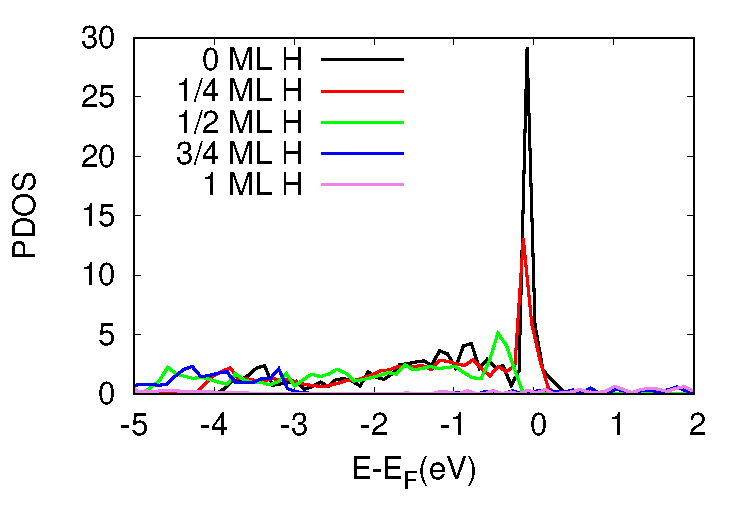
\includegraphics[width=0.65\linewidth]{Chap1/plots/DOS_ZnO_surfO.pdf}}\label{Chap:ZnO_H:fig:DOSO} 
  \\
  \subfigure[]{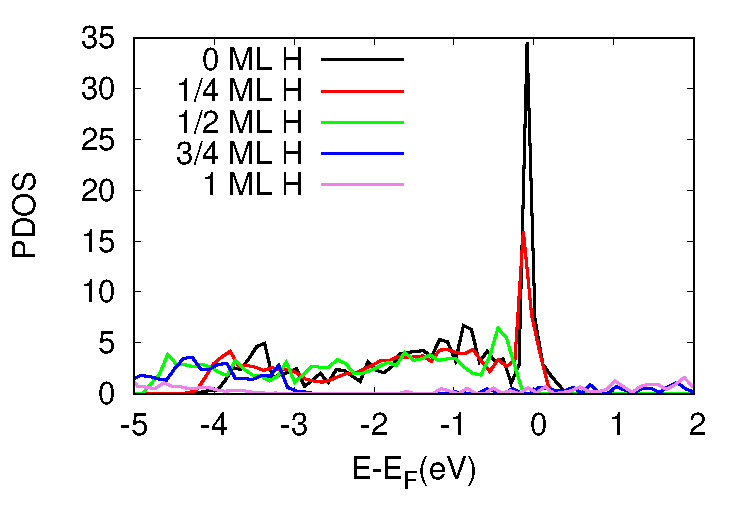
\includegraphics[width=0.65\linewidth]{Chap1/plots/DOS_ZnO_surface_all.pdf}}\label{Chap:ZnO_H:fig:DOSall}
  \caption[\ac{PDOS} for all the surface O atoms on pure ZnO (2$\times$2) (000$\overline{1}$) surface under different H coverage]{(a) \ac{PDOS} for all the surface O atoms on pure ZnO (2$\times$2) (000$\overline{1}$) surface under different H coverage. (b) \ac{PDOS} of all O, Zn and adsorbed H atoms on the topmost layer of ZnO (000$\overline{1}$) surface under different H coverage.}
  \label{Chap:ZnO_H:fig:DOS}
\end{figure}
\endgroup

The coincidence ($\frac{1}{2}$ \ac{ML}) of the critical $\theta_{\textup{H}}$ for the abrupt change of $E_{\textup{ad}}^{\textup{H}}$ and the critical $\theta_{\textup{H}}$ for the metal-semiconductor transition indicates that $E_{\textup{ad}}^{\textup{H}}$ is controlled by surface electronic structures. This coincidence can be explained by the electron counting model\cite{pashley1989electron}. Each Zn has 2 valence electrons, and each O has 6 valence electrons. In bulk wurtzite lattice, each Zn/O atom connects to 4 nearby O/Zn atoms so that every Zn-O bond has 2 valence electrons, in which 1.5 electrons are contributed from O and 0.5 electron is from Zn. After bulk ZnO is chopped into two slabs with two surfaces in [0001] direction, each surface O and Zn atom has one broken Zn-O bond, as shown in Fig. \ref{Chap:ZnO_H:fig:ZnO}. For Zn-terminated (0001) surface, we applied appropriate methods to passivate the dangling bonds as explained above. For O-terminated (000$\overline{1}$) surface, each O atom requires 0.5 more electron to fill its dangling bond and reach the closed-shell electron configuration. Thus, the electrons of clean O-terminated (000$\overline{1}$) surface are in open-shell configurations. 

The unpaired electrons from surface O atoms are delocalized, making ZnO surface in metallic states. There is a large energetic driving force for surface O atoms to reach closed-shell configurations, meaning ZnO surface has a strong adsorption strength to any atoms/molecules that can contribute electrons to surface O atoms, such as H. In a simple picture, each H atom can contribute one electron to make 2 surface O atoms on (000$\overline{1}$) ZnO surface transform into electron closed-shell configurations. Thus, once $\theta_{\textup{H}}$ reaches $\frac{1}{2}$ ML, there are no unpaired electrons in delocalized states on (000$\overline{1}$) ZnO surface. Correspondingly, the surface transforms into semiconductor state and has much weaker adsorption strength for the consecutive H atoms.

\begingroup
\begin{figure}[!ht]
  \centering
  \subfigure[]{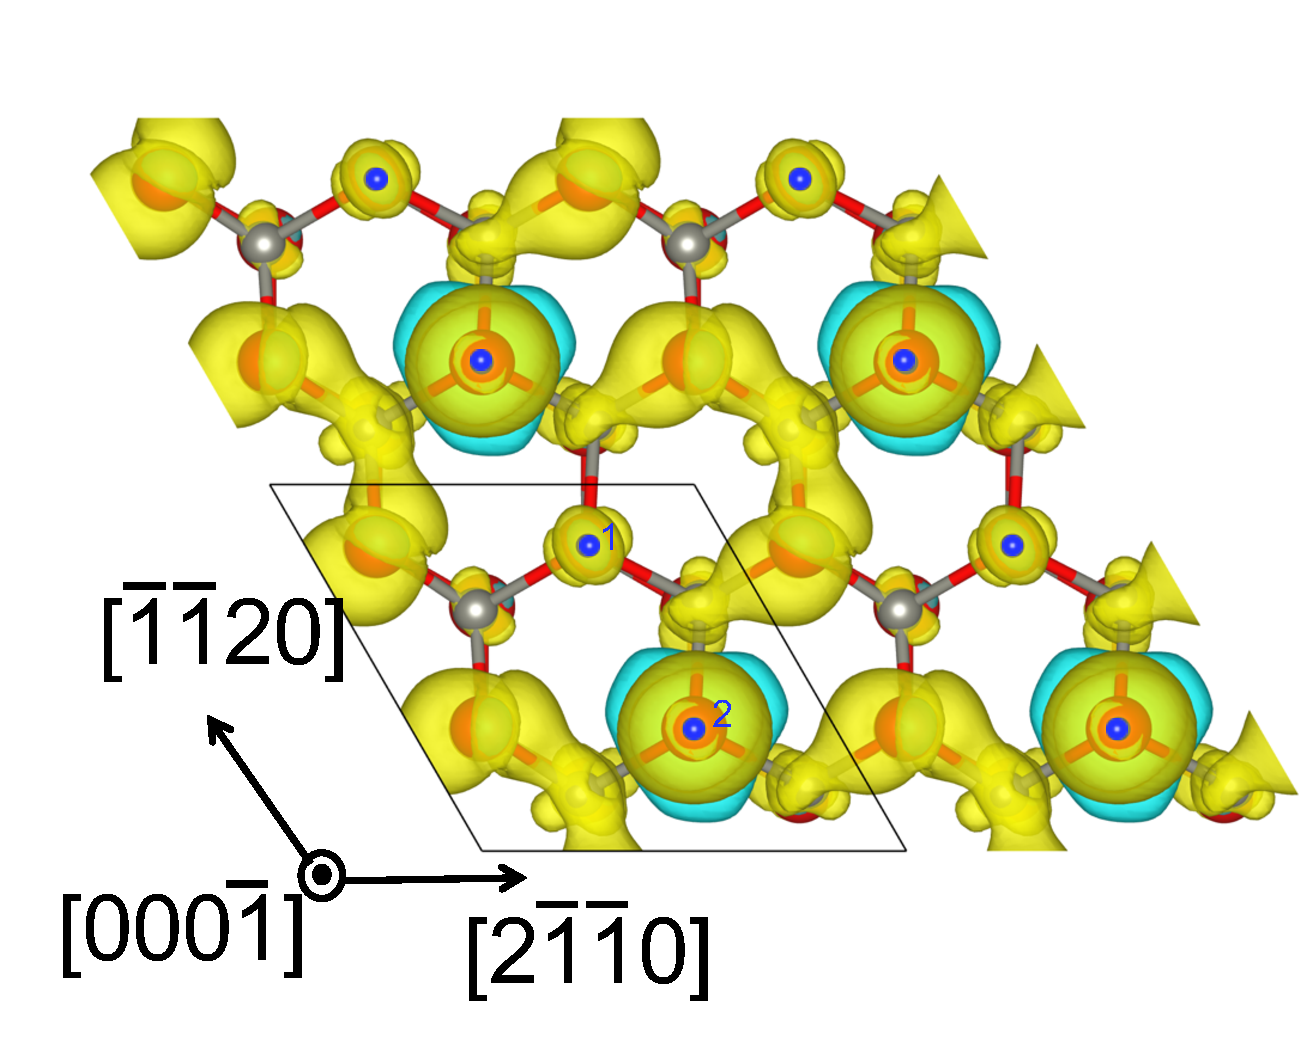
\includegraphics[width=0.55\linewidth]{Chap1/plots/chgdiff1.pdf}}\label{Chap:ZnO_H:fig:chgdiff1}
  \\
  \subfigure[]{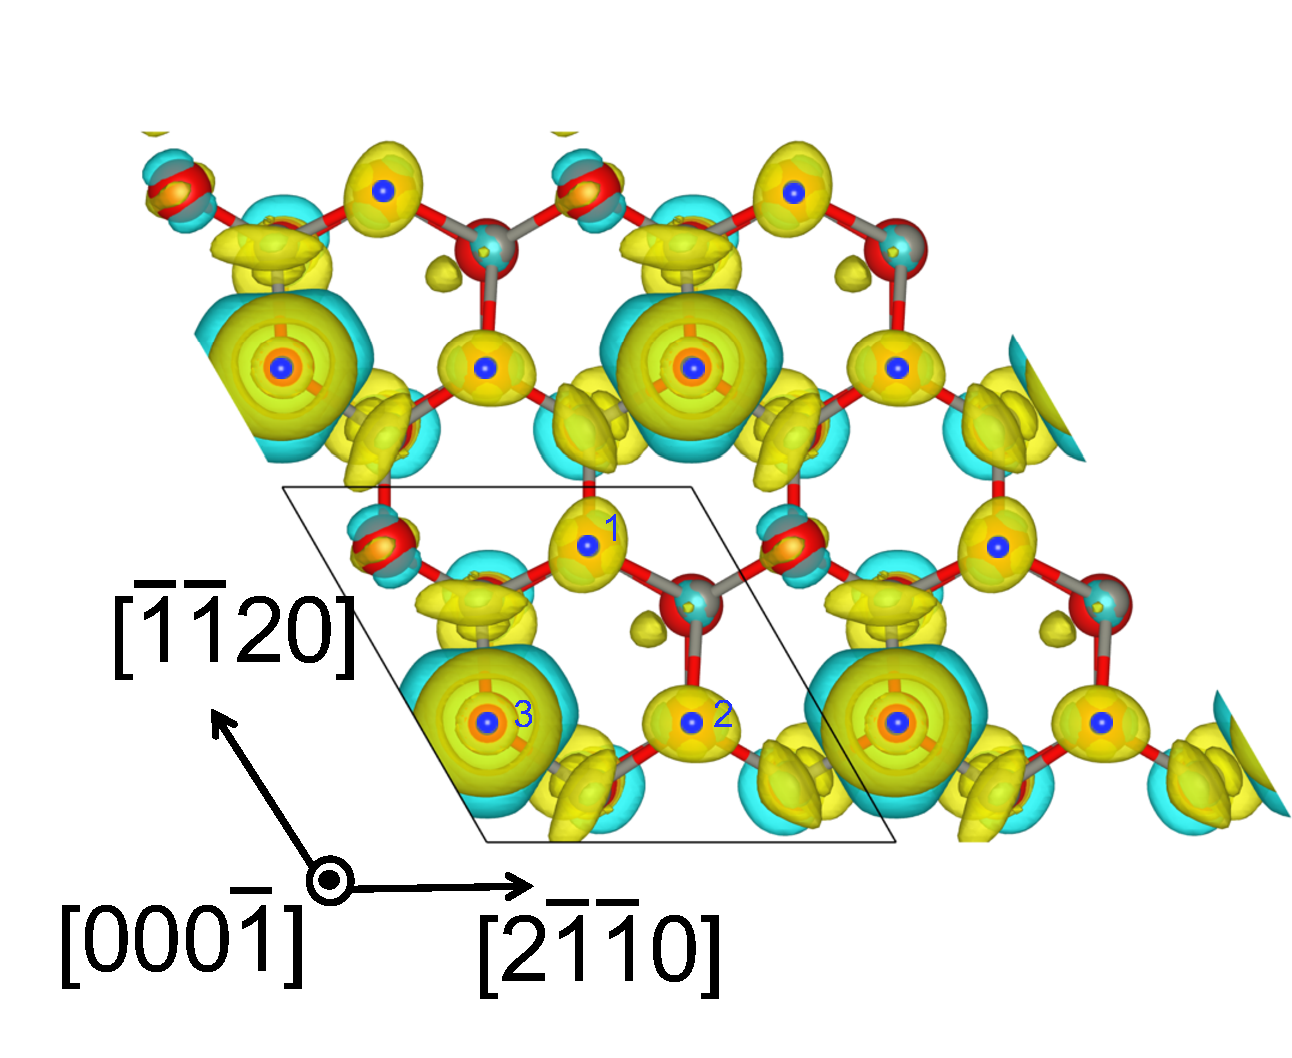
\includegraphics[width=0.55\linewidth]{Chap1/plots/chgdiff2.pdf}}\label{Chap:ZnO_H:fig:chgdiff2}
\caption[Top views of the charge density difference isosurfaces before and after H adsorption]{Top views of the charge density difference isosurfaces before and after (a) the second H and (b) the third adsorption on ZnO (000$\overline{1}$) surface in (2$\times$2) supercells, corresponding to $\Delta\rho(\theta_{\textup{H}}= \frac{1}{2} \textup{ ML})$ and $\Delta\rho(\theta_{\textup{H}}= \frac{3}{4} \textup{ ML})$ defined in Eq. \ref{eq2}, respectively. Large red, small grey and small blue atoms are O, Zn and H atoms, respectively. Label 1, 2 and 3 in the plots denote the adsorption site for the first, second, and third H atom, respectively. The yellow and blue color indicate electron accumulation and annihilation with the isosurface of $0.001e/{\textup{\AA}}^3$.}
  \label{fig3}
\end{figure}
\endgroup

Such electron counting rule and the corresponding \ac{PDOS} analyses can be further confirmed by the analyses of charge density difference on ZnO (000$\overline{1}$) surface due to H adsorption. Here we define the charge density difference $\Delta\rho$ at different $\theta_{\textup{H}}$ as the following
\begin{equation}
  \begin{array}{rcl}
    \Delta\rho(\theta_{\textup{H}}=\frac{n}{m}\textup{ML})&=&\rho(\textup{slab+}n\textup{H})-\rho(\textup{slab+}(n-1)\textup{H})
  \end{array}
  \label{eq2}
\end{equation}
Here $\rho(\textup{slab+}n \textup{H})$ and $\rho(\textup{slab+}(n-1) \textup{H})$ is the charge density of ZnO (000$\overline{1}$) surface slab with $n$ and $(n-1)$ adsorbed H atoms, respectively. For (2$\times$2) supercell, $\Delta\rho(\theta_{\textup{H}}= \frac{1}{2} \textup{ ML})$ and  $\Delta\rho(\theta_{\textup{H}}= \frac{3}{4} \textup{ ML})$ corresponds to the charge density difference induced by the adsorption of the second and third H atom in the supercell, as shown in Fig. \ref{Chap:ZnO_H:fig:chgdiff1} and  \ref{Chap:ZnO_H:fig:chgdiff2}, respectively. 

In Fig. \ref{Chap:ZnO_H:fig:chgdiff1}, the second H added on (2$\times$2) ZnO (000$\overline{1}$) surface induces charge density accumulation not only near this H atom itself but also other surface sites without H. Such delocalized $\Delta\rho$ is consistent with the metallic state of ZnO (000$\overline{1}$) surface with $\theta_{\textup{H}}$ $<$ $\frac{1}{2}$ \ac{ML}. The increase of charge density at multiple surface sites indicates that the electron from the second H atom intends to saturate the unpaired electrons on the whole surface and induce the metal-semiconductor transition. In Fig. \ref{Chap:ZnO_H:fig:chgdiff2}, the third H added on (2$\times$2) ZnO (000$\overline{1}$) surface results in charge density accumulation mostly located near the third H atom itself, with a localized s-orbital-like isosurface of $\Delta\rho$ shown in Fig. \ref{Chap:ZnO_H:fig:chgdiff2}. Such localized $\Delta\rho$ is consistent with the semiconductor electronic structure of ZnO (000$\overline{1}$) surface with $\theta_{\textup{H}}$ $\geq$ $\frac{1}{2}$ \ac{ML}.